\begin{mainquestion}{diodemodels}{Diode Circuit Analysis}

\questionpoints Consider the circuit below.

\begin{center}
    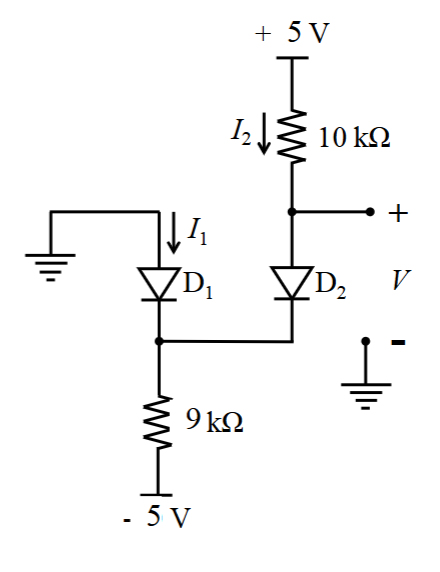
\includegraphics[width=0.4\textwidth]{diodes_voltage.png}
\end{center}

% =========================================================
\begin{partquestion}{ideal}
{Find the values of $I_1$, $I_2$, and the voltage $V$ assuming an \textbf{ideal diode model}.}

\begin{answer}
        \textbf{Assumption:} Assume both $D_1$ and $D_2$ are \textbf{ON}.
        \begin{itemize}
            \item If $D_1$ is ON (ideal), it acts as a short to ground. Therefore, the voltage at the junction node $V_B = 0\,\text{V}$.
            \item If $D_2$ is ON (ideal), it acts as a short. Therefore $V_A = V_B = 0\,\text{V}$.
            \item \textbf{Result for V:} $V = V_A = 0\,\text{V}$.
            \item \textbf{Currents:}
            \begin{itemize}
                \item $I_2 = \frac{5\,\text{V} - V_A}{10\,\text{k}\Omega} = \frac{5 - 0}{10} = 0.5\,\text{mA}$.
                \item The current leaving node B through the $9\,\text{k}\Omega$ resistor is $I_{load} = \frac{V_B - (-5\,\text{V})}{9\,\text{k}\Omega} = \frac{0 + 5}{9} \approx 0.556\,\text{mA}$.
                \item By KCL at node B: $I_1 + I_2 = I_{load} \implies I_1 = 0.556 - 0.5 = 0.056\,\text{mA}$.
            \end{itemize}
            \item \textbf{Check:} Since $I_1 > 0$ and $I_2 > 0$, our assumption that both diodes are ON is correct.
            \item \textbf{Final Answer:} $I_1 = 0.056\,\text{mA}$, $I_2 = 0.5\,\text{mA}$, $V = 0\,\text{V}$.
        \end{itemize}
\end{answer}

\end{partquestion}

% =========================================================
\begin{partquestion}{drop}
{Repeat part (a) using a \textbf{constant voltage drop model} with $V_D = 0.7\,\text{V}$.}

\begin{answer}
        \textbf{Assumption:} Let's first assume both are ON.
        \begin{itemize}
            \item $D_1$ ON $\implies V_B = 0\,\text{V} - 0.7\,\text{V} = -0.7\,\text{V}$.
            \item $D_2$ ON $\implies V_A = V_B + 0.7\,\text{V} = 0\,\text{V}$.
            \item $I_2 = \frac{5 - 0}{10\,\text{k}\Omega} = 0.5\,\text{mA}$.
            \item $I_{load} = \frac{-0.7 - (-5)}{9\,\text{k}\Omega} = \frac{4.3}{9} \approx 0.478\,\text{mA}$.
            \item KCL: $I_1 + I_2 = I_{load} \implies I_1 = 0.478 - 0.5 = -0.022\,\text{mA}$.
            \item \textbf{Contradiction:} $I_1$ cannot be negative. Thus, $D_1$ must be \textbf{OFF}.
        \end{itemize}
        
        \textbf{New Assumption:} $D_1$ is OFF, $D_2$ is ON.
        \begin{itemize}
            \item $I_1 = 0\,\text{A}$.
            \item The circuit is a single series loop: $+5\,\text{V} \to 10\,\text{k}\Omega \to D_2 \to 9\,\text{k}\Omega \to -5\,\text{V}$.
            \item KVL: $5 - 10 I_2 - 0.7 - 9 I_2 - (-5) = 0$.
            \item $10 - 0.7 + 5 - 5 = 19 I_2 \implies 9.3 = 19 I_2$.
            \item $I_2 = \frac{9.3}{19} \approx 0.489\,\text{mA}$.
            \item \textbf{Voltage V:} $V = 5 - 10(0.489) = 5 - 4.89 = 0.11\,\text{V}$.
            \item \textbf{Check $D_1$:} $V_B = V - 0.7 = 0.11 - 0.7 = -0.59\,\text{V}$. The anode of $D_1$ is at ground ($0\,\text{V}$). For $D_1$ to turn on, we need $V_{Anode} - V_{Cathode} \ge 0.7$. Here, $0 - (-0.59) = 0.59\,\text{V} < 0.7\,\text{V}$. So $D_1$ stays OFF.
            \item \textbf{Final Answer:} $I_1 = 0\,\text{A}$, $I_2 = 0.489\,\text{mA}$, $V = 0.11\,\text{V}$.
        \end{itemize}
\end{answer}

\end{partquestion}

% =========================================================
\begin{partquestion}{level}
{If you were to lower the diode's forward voltage below $0.7\,\text{V}$, at what voltage level will the operating state of $D_1$ and/or $D_2$ first change?}

\begin{answer}
        The state changes when $D_1$ turns ON.
        \begin{itemize}
            \item Condition for $D_1$ turn-on: $V_{Anode} - V_{Cathode} = V_D$.
            \item Since $V_{Anode} = 0V$, this requires $V_B = -V_D$.
            \item Since $D_2$ is already ON, $V_A = V_B + V_D = -V_D + V_D = 0\,\text{V}$.
            \item If $V_A = 0\,\text{V}$, then current $I_2 = \frac{5\,\text{V} - 0\,\text{V}}{10\,\text{k}\Omega} = 0.5\,\text{mA}$.
            \item Since $D_1$ is just turning on, $I_1 = 0A$, so all current flows through the $9\,\text{k}\Omega$ resistor.
            \item $I_{load} = \frac{V_B - (-5\,\text{V})}{9\,\text{k}\Omega} = \frac{-V_D + 5\,\text{V}}{9\,\text{k}\Omega}$.
            \item Equating currents ($I_2 = I_{load}$):
            \[ 0.5\,\text{mA} = \frac{5\,\text{V} - V_D}{9\,\text{k}\Omega} \]
            \[ 4.5\,\text{V} = 5\,\text{V} - V_D \implies V_D = 0.5\,\text{V} \]
        \end{itemize}
        Thus, if the forward voltage drops below $0.5\,\text{V}$, $D_1$ will turn on.
\end{answer}

\begin{comment}
    \item \textbf{EXTRA CREDIT:} Replacing the $10\,\text{k}\Omega$ resistor with a generic $R_1$, the $9\,\text{k}\Omega$ resistor with a generic $R_2$, and the $\pm 5\,\text{V}$ DC power supplies with a generic $\pm V_{CC}$, find the expression for $V_D$ that answers part (c) above. (5 points)

\begin{answer}
        Using the logic from part (c), the transition occurs when $V_A = 0\,\text{V}$.
        \begin{itemize}
            \item $I_2 = \frac{V_{CC} - V_A}{R_1} = \frac{V_{CC}}{R_1}$.
            \item $V_B = V_A - V_D = -V_D$.
            \item $I_{load} = \frac{V_B - (-V_{CC})}{R_2} = \frac{V_{CC} - V_D}{R_2}$.
            \item Equating $I_2 = I_{load}$:
            \[ \frac{V_{CC}}{R_1} = \frac{V_{CC} - V_D}{R_2} \]
            \[ R_2 V_{CC} = R_1 V_{CC} - R_1 V_D \]
            \[ R_1 V_D = V_{CC} (R_1 - R_2) \]
            \[ V_D = V_{CC} \left( 1 - \frac{R_2}{R_1} \right) \]
        \end{itemize}
        (Checking with part c values: $5(1 - 9/10) = 5(0.1) = 0.5\,\text{V}$. Correct.)
\end{answer}

\end{comment}
\end{partquestion}

\end{mainquestion}
